\documentclass[a4paper,11pt]{article}
%\usepackage[utf8]{inputenc}

\usepackage{pdfpages}
\usepackage{mathtools}
\usepackage{amsmath}
\usepackage{amssymb}
\usepackage{tikz}
\usepackage{physics}
\usepackage{listings}

\newcommand{\Mypm}{\mathbin{\tikz [x=1.4ex,y=1.4ex,line width=.1ex] \draw (0.0,0) -- (1.0,0) (0.5,0.08) -- (0.5,0.92) (0.0,0.5) -- (1.0,0.5);}}%


\newcommand\underrel[3][]{\mathrel{\mathop{#3}\limits_{%
      \ifx c#1\relax\mathclap{#2}\else#2\fi}}}

\numberwithin{equation}{section}
\numberwithin{figure}{section}
\usepackage{graphicx}
\setlength{\parindent}{0cm}

\title{\Huge \textbf{Dhoni's Magnificience}}
\author{\Large Riddhiman Bhattacharya}
\date{}

\usepackage{geometry}
\geometry{a4paper, left=25mm, right=25mm, top=30mm, bottom=25mm}

\renewcommand{\baselinestretch}{1.2}

\begin{document}


\clearpage
\maketitle
\thispagestyle{empty}


\large

\section{Problem}
In a moment that will forever be etched in cricketing history, the legendary M.S. Dhoni, at Wankhede Stadium, with nerves of steel and unwavering determination, unleashed his full power and mastery. The roaring crowd held their breath as the ball soared high into the night sky, defying gravity itself. With the weight of an entire nation's hopes on his shoulders, Dhoni's bat connected with the leather, sending it on a trajectory of glory. The ball collided with the stadium roof, releasing an electrifying surge of emotion, sealing India's momentous World Cup victory with an explosion of force.
Now as a Physics Student, calculate With what force does the ball hit the roof of the stadium.


\section{Solution}
To determine the force (or possibly momentum, energy, etc.) with which the ball hits the roof, we first need to determine the point and velocity at which the ball hits the roof. We'll initially neglect any influences from the wind, but consider the effects of air friction on the ball as well as the force of gravity. Let $v(t) = (v_x(t), v_y(t))^T$ represent the velocity of the ball at time $t$, and let $\tan \alpha = \frac{v_y}{v_x}$. The air friction force $F_R$ always acts against the direction of the ball's motion. We'll decompose this frictional force into its $x$ and $y$ components, and the forces $F_x$ and $F_y$ acting on the ball will be given by: $F_x = -F_R \cos \alpha$ and $F_y = -(F_R \sin \alpha + F_G)$, where $F_G$ is the force of gravity.

Applying Newton's $2^\text{nd}$ law, $F = ma$, we can find the $x$-component acceleration $a_x$ of the ball (with $k = \frac{1}{2}c_w \rho A$ and $\kappa = \frac{k}{m}$, where $c_w$ is the drag coefficient, $\rho$ is the air density, $A$ is the cross-sectional area of the ball, and $m$ is the mass of the ball):

\begin{align*}
    a_x        & = -\frac{F_R \cos \alpha}{m}                                      \\
    \implies -ma_x & = k \norm{v}^2 \cos \alpha                                        \\
    \implies 0     & = \kappa (v_x^2 + v_y^2) \cos \arctan \frac{v_y}{v_x} + \dot{v}_x
\end{align*}

Similarly, for the $y$-component acceleration $a_y$:

\begin{align*}
    a_y        & = -\frac{F_R \sin \alpha + F_G}{m}                                     \\
    \implies -ma_y & = k \norm{v}^2 \sin \alpha + m g                                       \\
    \implies 0     & = \kappa (v_x^2 + v_y^2) \sin \arctan \frac{v_y}{v_x} + g + \dot{v}_y
\end{align*}

Therefore, the system of differential equations to solve are:

\begin{align*}
    0 & = \kappa (v_x^2 + v_y^2) \cos \arctan \frac{v_y}{v_x} + \dot{v}_x     \\
    0 & = \kappa (v_x^2 + v_y^2) \sin \arctan \frac{v_y}{v_x} + \dot{v}_y + g
\end{align*}

subject to the initial conditions $v_x(0), v_y(0) \in \mathbb{R}$.

Let, $$h := \left(
    \begin{array}{c}
            x       \\
            y       \\
            \dot{x} \\
            \dot{y} \\
        \end{array}
    \right) \implies \dot{h} = \left(
    \begin{array}{c}
            \dot{x}  \\
            \dot{y}  \\
            \ddot{x} \\
            \ddot{y} \\
        \end{array}
    \right)$$
with $v_x = \dot{x}$ and $v_y = \dot{y}$. Then, we can rewrite the above initial value problem as:

$$
    \dot{h} = f(t,h) = f(t, (x, y, \dot{x}, \dot{y})^T) = \left( \begin{array}{c}
            \dot{x}                                                                                            \\
            \dot{y}                                                                                            \\
            -\frac{\kappa(\dot{x}^2 + \dot{y}^2)}{\sqrt{(\frac{\dot{y}}{\dot{x}})^2+1}}                        \\
            -(\frac{\kappa \dot{y} (\dot{x}^2 + \dot{y}^2)}{\dot{x} \sqrt{(\frac{\dot{y}}{\dot{x}})^2+1}} + g) \\
        \end{array} \right)
$$
\newpage
\section{Code}

\lstset{
    language=Python,
    basicstyle=\ttfamily\small,
    columns=fixed,
    extendedchars=true,
    breaklines=true,
    tabsize=4,
    numbers=none, % Remove line numbers here
    captionpos=t,
    escapeinside={\%*}{*)}
}

\lstinputlisting{Plots.py}

\newpage
\section{Plot}

\begin{figure}[h]
    \centering
    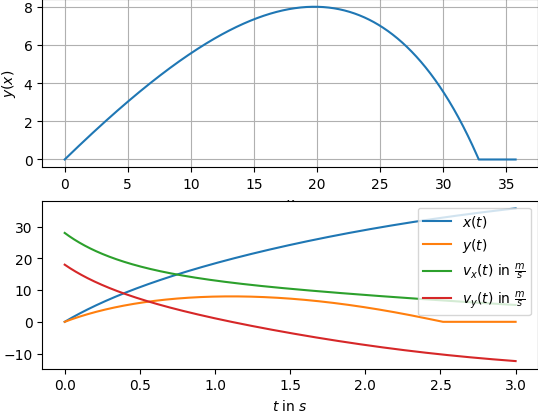
\includegraphics{Plot.png}
    \caption{\small
\textbf{Top Plots}:
Y-axis: $y(x)$ (Vertical position of the object with respect to horizontal position $x$).
X-axis: $x$ (Horizontal position of the object).\\
\textbf{Bottom Plots}
Blue:
Y-axis: $x(t)$ (Horizontal position of the object with respect to time $t$).
X-axis: $t$ (Time).\\
Orange:
Y-axis: $y(t)$ (Vertical position of the object with respect to time $t$).
X-axis: $t$ (Time).\\
Green:
Y-axis: $v_x(t)$ (Horizontal velocity of the object with respect to time $t$) in $\frac{m}{s}$.
X-axis: $t$ (Time).\\
Red:
Y-axis: $v_y(t)$ (Vertical velocity of the object with respect to time $t$) in $\frac{m}{s}$.
X-axis: $t$ (Time).}

\end{figure}

\end{document}